\section{Rebuilders}\label{sec-rebuilder}

A build system can be split into a scheduler (as defined
in~\S\ref{sec-scheduler}) and a \emph{rebuilder}. Suppose the scheduler decides
that a key should be brought up to date. The next question is: does any work
need to be done, or is the key already up to date? Or, in a cloud build system,
do we have a cached copy of the value we need?

While~\S\ref{sec-background} explicitly listed the schedulers, the rebuilders
were introduced more implicitly, primarily by the information they retain to
make their decisions. From the examples we have looked at we see four
fundamental rebuilders, each with a number of tweaks and variations within them.

\subsection{A Dirty Bit}\label{sec-dirty-bit}

The idea of a dirty bit is to have one piece of persistent information per key,
saying whether the key is \emph{dirty} or \emph{clean}. After a build, all bits
are set to clean. When the next build starts, anything that changed between the
two builds is marked dirty. If a key and all its transitive dependencies are
clean, the key does not need to be rebuilt. Taking the example from
Fig.~\ref{fig-make}(c), if \cmd{main.c} changes then it would be marked dirty,
and \cmd{main.o} and \cmd{main.exe} would be rebuilt as they transitively depend
on \cmd{main.c}.

\Excel models the dirty bit approach most directly, having an actual dirty bit
associated with each cell, marking the cell dirty if the user modifies it.
It also marks dirty all cells that (transitively) depend on the modified cell.
\Excel does not record dynamic dependencies of each cell; instead it computes a
\emph{static over-approximation} -- it is safe for it to make more cells dirty
than necessary, but not vice versa. The over-approximation is as follows: a cell
is marked dirty (i) if its formula statically refers to a dirty cell, or (ii) if
the formula calls a \emph{volatile} function like \cmd{INDIRECT} whose
dependencies cannot be guessed from the formula alone. The over-approximation is
clear for \cmd{INDIRECT}, but it is also present for \cmd{IF}, where both
branches are followed even though dynamically only one is used.

\Make uses file modification times, and compares files to their dependencies,
which can be thought of as a dirty bit which is set when a file is older than
its dependencies. The interesting property of this dirty bit is that it is not
under the control of \Make; rather it is existing file-system information that
has been repurposed. Modifying a file automatically clears its dirty bit, and
automatically sets the dirty bit of the files depending on it (but not
recursively). Note that \Make requires that file timestamps only go forward in
time, which can be violated by backup software.

With a dirty bit it is possible to achieve
minimality~(\S\ref{sec-background-make}). However, to achieve early
cutoff~(\S\ref{sec-background-shake}) it would be important to clear the dirty
bit after a computation that did not change the value and make sure that cells
that depend on it are not rebuilt unnecessarily. For \Excel, this is difficult
because the dependent cells have already been recursively marked dirty. For
\Make, it is impossible to mark a file clean and at the same time not mark the
keys that depend on it dirty. \Make can approximate early cutoff by not
modifying the result file, and not marking it clean, but then it will be rebuilt
in every subsequent build.

A dirty bit rebuilder is useful to reduce memory consumption, and in the case
of \Make, to integrate with the file system. However, as the examples show, in
constrained environments where a dirty bit is chosen, it is often done as part
of a series of compromises.

It is possible to write a dirty-bit builder which is minimal and supports early
cutoff. To do so, you need to start with all inputs that have changed marked dirty,
then a node must be rebuilt if any children are dirty, and must set that node to dirty
only if the result changes. At the end of the build all dirty bits
must be reset to not-dirty. This approach only works if all targets are rebuilt each time,
since clearing dirty bits of children who aren't targets will cause them to incorrectly
not rebuild subsequently. To avoid resetting the dirty bit,
it is possible to use successive execution numbers, which ultimately leads to an approach
we call verifying step traces in \S\ref{sec-step-traces}.

\subsection{Verifying Traces}\label{sec-verifying-traces}

An alternative way to determine if a key is dirty is to record the
values/hashes of dependencies used last time, and if something has changed, the
key is dirty and must therefore be rebuilt~--~in essence, keeping a \emph{trace}
which we can use to \emph{verify} existing values. Taking the example from
Fig.~\ref{fig-bazel}(c), we might record that the key \cmd{util.o} (at hash 8)
depended on the keys \cmd{util.c} (at hash 7) and \cmd{util.h} (at hash 2). Next
time round, if the scheduler decides that it is time for \cmd{util.o} to be
rebuilt and all keys still have the same hashes as in the recorded trace, there
is nothing to do, and we can skip rebuilding. If any of the hashes is different,
we rebuild \cmd{util.o}, and record a trace with the new values.

For traces, there are two essential operations~--~adding a new trace to the
trace store, and using the traces to determine if a key needs rebuilding.
Assuming a store of verifying traces \hs{VT}~\hs{k}~\hs{v}, the operations are:

\vspace{1mm}
\begin{minted}[xleftmargin=10pt]{haskell}
recordVT :: k -> Hash v -> [(k, Hash v)] -> VT k v -> VT k v
\end{minted}
\vspace{-2mm}
\begin{minted}[xleftmargin=10pt]{haskell}
verifyVT :: (Monad m, Eq k, Eq v)
         => k -> Hash v -> (k -> m (Hash v)) -> VT k v -> m Bool
\end{minted}
\vspace{1mm}

\noindent
Rather than storing (large) values \hs{v}, the verifying trace \hs{VT} can store
only hashes, of type \hs{Hash}~\hs{v}, of those values. Since the verifying
trace persists from one build to the next -- it constitutes the build system's
``memory'' -- it is helpful for it to be of modest size. After successfully
building a key, we call \hs{recordVT} to add a record to the current \hs{VT},
passing the key, the hash of its value, and the list of hashes and dependencies.

More interestingly, to \emph{verify} whether a key needs rebuilding we use
\hs{verifyVT}, supplying the key, the hash of its current value, a function for
obtaining the hash of the post-build value of any key (using a scheduling
strategy as per~\S\ref{sec-scheduler}), and the existing trace store \hs{VT}.
The result will be a \hs{Bool} where \hs{True} indicates that the current value
is already up to date, and \hs{False} indicates that it should be rebuilt.

The most complex argument of \hs{verifyVT} is a function
\hs{fetchHash}~\hs{::}~\hs{k}~\hs{->}~\hs{m}~\hs{(Hash}~\hs{v)} to obtain the
hash of the post-build value of any key. With an applicative task,
\hs{fetchHash} will be called on the statically known task dependencies.
However, with a monadic task, the dependencies are not known from the task
alone, they are only recorded from previous executions and stored in \hs{VT}. If
the build system has two traces for a given key~\hs{k}, they will both request
the same dependency first, since \hs{Task}~\hs{Monad} is deterministic. However,
depending on that first result, they may then request different successive
dependencies using \hs{fetchHash}. A curious result is that for suspending
schedulers~(\S\ref{sec-suspending}) in many cases the actual build steps are
performed as a consequence of checking if a key needs rebuilding!

A verifying trace, and other types of traces discussed in this section, support
dynamic dependencies and minimality; furthermore, all traces except for deep
traces~(\S\ref{sec-deep-constructive-traces}) support the early cutoff
optimisation~(\S\ref{sec-background-shake}).

\subsubsection{Trace Representation}

One potential implementation would be to record all arguments passed to
\hs{recordVT} in a list, and verify by simply checking if any list item matches
the information passed by \hs{verifyVT}. Concretely, in our implementations
from~\S\ref{sec-implementations}, traces are recorded as lists of:

\vspace{1mm}
\begin{minted}[xleftmargin=10pt]{haskell}
data Trace k v a = Trace { key     :: k
                         , depends :: [(k, Hash v)]
                         , result  :: a }
\end{minted}
\vspace{1mm}

\noindent
Where \hs{a} is \hs{Hash}~\hs{v} for verifying traces (and \hs{v} for
constructive traces, discussed later in~\S\ref{sec-constructive-traces}). A real
system is highly likely to use a more optimised implementation.

The first optimisation is that any system using \hs{Applicative} dependencies
can omit the dependency keys from the \hs{Trace} since they can be recovered
from the \hs{key} field~(\S\ref{sec-deps}).

The next optimisation is that there is only very minor benefit from storing more
than one \hs{Trace} per key. Therefore, verifying traces can be stored as
\hs{Map}~\hs{k}~\hs{(Trace}~\hs{k}~\hs{v}~\hs{(Hash}~\hs{v))}, where the
initial \hs{k} is the \hs{key} field of \hs{Trace}, thus making \hs{verifyVT}
much faster. Note that storing only one \hs{Trace} per key means that if the
dependencies of a key change but the resulting value does not, and then the
dependencies change back to what they were before, there will be no valid
\hs{Trace} available and the key will therefore have to be rebuilt, whereas a
complete list of all historical traces would allow the rebuilding to be skipped.
On the other hand, bounding the number of \hs{Trace} structures by the number of
distinct keys, regardless of how many builds are executed, is a useful property.

\subsubsection{Verifying Step Traces}\label{sec-step-traces}

The \Shake build system and the associated paper -- see~\S2.3.3
in~Mitchell~\shortcite{mitchell2012shake} -- use a slightly different trace
structure, called \emph{step traces}, one that is similar to verifying traces,
but stores less data, and has different early cutoff semantics. Rather than
storing the \hs{Hash}~\hs{v} for each dependency, it instead stores \hs{built}
time and \hs{changed} time for the \hs{key}, and a list of dependency keys
(without the hashes). The resulting \hs{StepTrace} type resembles:

\vspace{1mm}
\begin{minted}[xleftmargin=10pt]{haskell}
data StepTrace k v = StepTrace { key     :: k
                               , result  :: Hash v
                               , built   :: Time
                               , changed :: Time
                               , depends :: [k] }
\end{minted}
\vspace{1mm}

\noindent
The \hs{built} field is when the \hs{key} last rebuilt. The \hs{changed} field
is when the \hs{result} last changed -- if the last build changed the value, it
will be equal to \hs{built}, otherwise it will be older. The function
\hs{recordVT} consults the previous step traces to know whether to keep the
previous \hs{changed} value or change it to \hs{built}. The function
\hs{verifyVT} is a bit more subtle; given a key \hs{k} and the hash of its
current value \hs{h}, it performs the following steps:

\begin{itemize}
\item Find the latest (with respect to the field \hs{built}) step trace matching
  \hs{k}. If it does not exist, return \hs{False}: \hs{k} was never built
  before and cannot be verified.
\item If \hs{h} does not equal the \hs{result} field of the trace, return
  \hs{False}: the current \hs{k}'s value was written externally and needs
  rebuilding.
\item For each key \hs{d} in \hs{depends}:\\
  $\circ$ Make sure \hs{d} is up-to-date, suspending the current task if needed;\\
  $\circ$ If \hs{d}'s latest \hs{changed} time is greater than \hs{k}'s
    \hs{built} time, return \hs{False}.
\item Return \hs{True}: the current \hs{k}'s value is up-to-date.
\end{itemize}

\noindent
This approach preserves minimality and early cutoff. A variant with only one
\hs{Time} field would lose early cutoff, and indeed corresponds quite closely to
\Make. Furthermore, the \hs{Time} stamp only needs to record which execution of
the build is running, so every key built in the same run can share the same
\hs{Time} value -- it just needs to be monotonically increasing between runs.

This optimisation is useful, at least in the case of \Shake, to save space. A
typical cryptographic hash takes up 32 bytes, while a key (in \Shake only) is an
\hs{Int} taking only~4~bytes. Furthermore, \Shake permits values to be
arbitrarily large, and permits a custom equality (two values can be bit-for-bit
unequal but considered equal by \Shake), meaning that a \hs{Hash} is not a valid
encoding. For build systems that use \hs{Applicative} dependencies, the
\hs{depends} could be omitted entirely, making the size of a \hs{StepTrace}
$O(1)$ instead of $O(n)$, where $n$ is the number of dependencies.

\begin{figure}%[h]
\begin{subfigure}[b]{0.32\linewidth}
\centerline{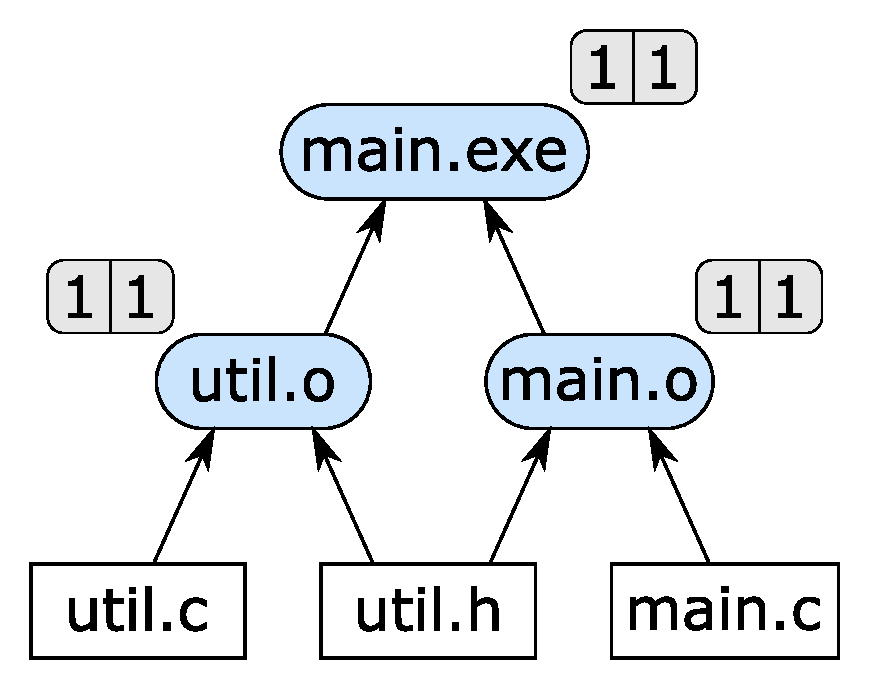
\includegraphics[scale=0.28]{fig/step-example-step1.pdf}}
\caption{Initial full build}
\end{subfigure}
\hfill
\begin{subfigure}[b]{0.32\linewidth}
\centerline{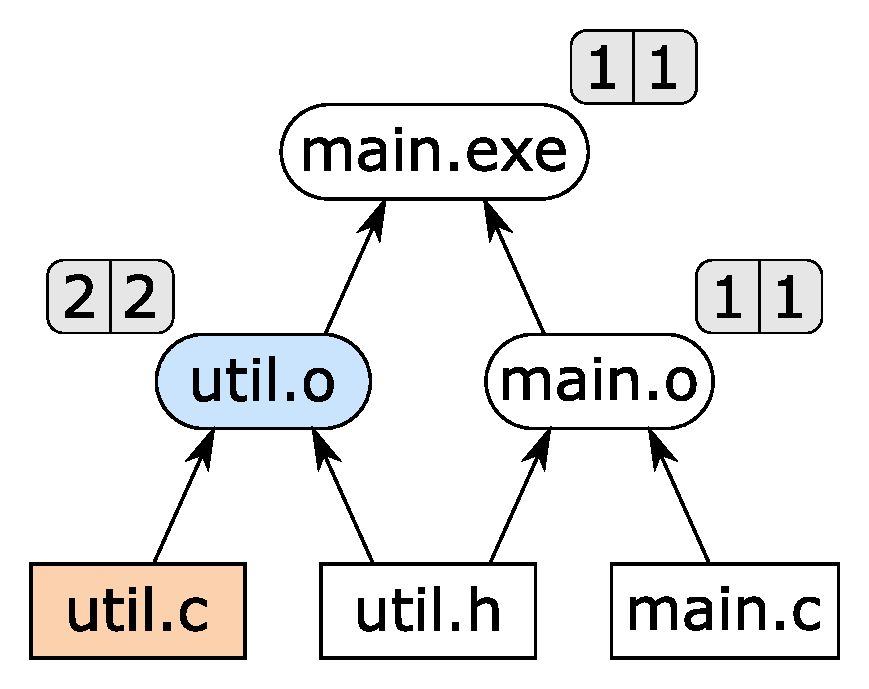
\includegraphics[scale=0.28]{fig/step-example-step2.pdf}}
\caption{Change \cmd{util.c}, build \cmd{util.o}}
\end{subfigure}
\hfill
\begin{subfigure}[b]{0.33\linewidth}
\centerline{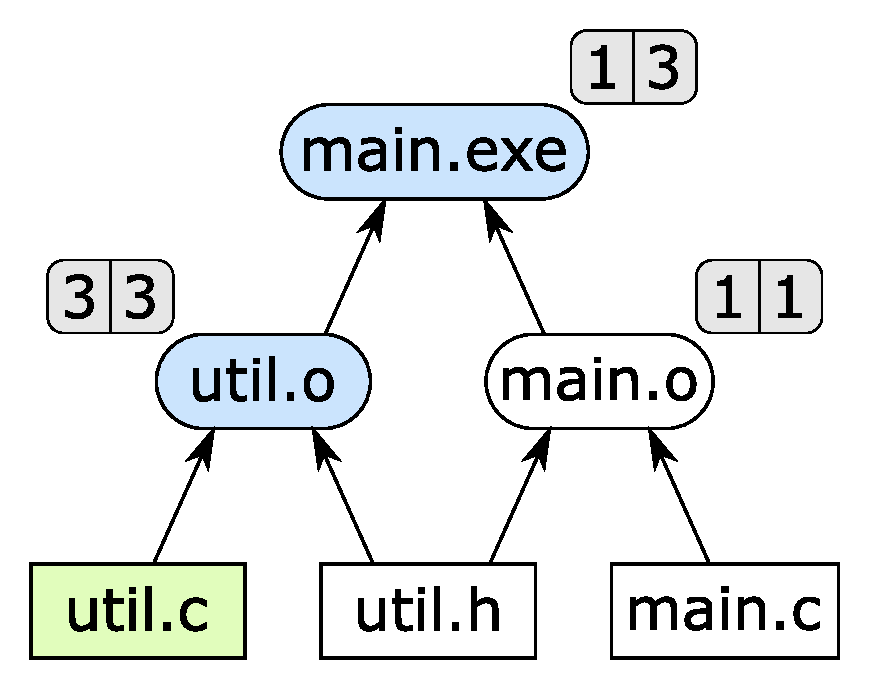
\includegraphics[scale=0.28]{fig/step-example-step3.pdf}}
\caption{Restore \cmd{util.c}, build \cmd{main.exe}}
\end{subfigure}
% \vspace{-2mm}
\caption{An example of verifying step traces. The small rectangles show the
\hs{changed} (left) and \hs{built} (right) timestamps of each non-input key
in the trace store.
\label{fig-step}}
% \vspace{-2mm}
\end{figure}

While verifying step traces are mostly an optimisation, there are some
observable differences from verifying traces, as demonstrated by an example in
Fig.~\ref{fig-step}. We first make the full build: all keys get a \hs{built} and
\hs{changed} of timestamp 1. Next we change \cmd{util.c} and build \cmd{util.o};
the latter is changed as a result and hence both \hs{built} and \hs{changed} are
increased to 2. Finally, we change \cmd{util.c} back to what it was originally,
and build \cmd{main.exe}. With verifying traces, the hashes of the dependencies
of \cmd{main.exe} would be equal to the initial build, and \cmd{main.exe} would
not need rebuilding. With verifying step traces, the \hs{changed} field of
\cmd{util.o} would increase once more, and \cmd{main.exe} would therefore be
rebuilt. As shown in Fig.~\ref{fig-step}(c), the \hs{changed} field of
\cmd{main.exe} remains 1, since the actual value is unchanged. Other than when
building subsets of the targets, we are unaware of any other situation where
verifying step traces are less powerful.

\subsection{Constructive Traces}\label{sec-constructive-traces}

A verifying trace deliberately records only small hashes, so that it can be small.
In contrast, a \emph{constructive} trace also stores the resulting value. Concretely,
it records a list of \hs{Trace}~\hs{k}~\hs{v}.
Once we are storing the complete result it makes sense
to record many constructive traces per key, and to share them with other users,
providing cloud-build functionality. We can represent this additional
information with the operations:

\begin{minted}[fontsize=\small,xleftmargin=10pt]{haskell}
recordCT    :: k -> v -> [(k, Hash v)] -> CT k v -> CT k v
constructCT :: (Monad m, Eq k, Eq v)
            => k -> (k -> m (Hash v)) -> CT k v -> m [v]
\end{minted}

\noindent
The function \hs{recordCT} looks like \hs{recordVT}, but instead of just passing
the hash of the resulting value, we require the actual value. The \hs{verifyVT}
has been replaced with \hs{constructCT}, which instead of taking the hash of the
current value as \emph{input}, returns a list of suitable values as \emph{output}.
If the current value in the store matches one of the possible values, the build
can skip this key. If the resulting list is empty, the key must be rebuilt.
However, if the current value does not match the store, and there is a possible
value, we can use any value from the constructive list \emph{without} doing any
work to build it, and copy it into the store.

Any \hs{Applicative} build system using constructive traces, e.g.
\CloudBuild, can index directly from the key and results to the output result~--~i.e.
\hs{Map}~\hs{(@@k,}~\hs{[Hash}~\hs{v])}~\hs{v}. Importantly, assuming the traces
are stored on a central server, the client can compute the key and the hashes of
its dependencies, then make a single call to the server to retrieve the result.

In practice, many cloud build systems store hashes of values in the trace information,
then have a separate content-addressable cache which associates hashes with
their actual contents.

\subsection{Deep Constructive Traces}\label{sec-deep-constructive-traces}

Constructive traces always verify keys by looking at their immediate
dependencies, which must have first been brought up to date, meaning that the
time to verify a key depends on the number of transitive dependencies. A
\emph{deep} constructive trace optimises this process by only looking at the
terminal \emph{input keys}, ignoring any intermediate dependencies. The operations
capturing this approach are the same as for constructive traces
in~\S\ref{sec-constructive-traces}, but we use the names \hs{recordDCT} and
\hs{constructDCT}, where the underlying \hs{DCT} representation need only record
information about hashes of inputs, not intermediate dependencies.

Concretely, taking the example from Figure \ref{fig-make}, to decide whether \hs{main.exe}
is out of data, a \emph{constructive} trace would look at \hs{util.o} and \hs{main.o}
(the immediate dependencies), while a \hs{deep constructive} trace would look at \hs{util.c},
\hs{util.h} and \hs{main.c}.

An advantage of deep constructive traces is that to decide if \hs{main.exe} is up to date only
requires consulting its inputs, not even considering \hs{util.o} or \hs{main.o}.
Such a feature is often known as a \emph{shallow build}, as discussed in~\S\ref{sec-cloud-aspects}.

There are two primary disadvantages of deep constructive traces:

\begin{description}
\item[Deterministic tasks] If the tasks are not \emph{deterministic} then it is possible to
violate correctness, as illustrated by an example in~\S\ref{sec-cloud-aspects}
(see Fig.~\ref{fig-frankenbuild}).
\item[No early cutoff] Such traces cannot support early cutoff
(\S\ref{sec-background-shake}), since the results of intermediate computations are not considered.
\end{description}

Current build systems using deep constructive traces always record hashes of
terminal \emph{input keys}, but the technique works equally well if we skip any
number of dependency levels (say $n$ levels). The input-only approach is the
special case of $n = \infty$, and constructive traces are the special case of
$n = 1$. By picking values of $n$ in between we would regain some early cutoff, at the
cost of losing such simple shallow builds and still requiring determinstic tasks.
